\chapter{Propuesta}\label{chapter:proposal}
El enfoque utilizado en este trabajo es la traducción automática basada
en aprendizaje de máquinas, abordada en la subsección \ref{subsection:state-of-the-art:traduccion:maquina} y la combinación de redes convolucionales y redes LSTM mencionado en las subsecciones \ref{subsection:state-of-the-art:slp:CNN}  y \ref{subsection:state-of-the-art:slp:LSTM} .
Se decidió utilizar dicha combinación puesto que los métodos del estado del arte basados en transformadores, pese a dar buenos resultados, requieren una cantidad exhorbitante de datos, de buena calidad y bien anotados, a diferencia de los datos que el autor emplea en este trabajo, de los cuales se abordará más adelante. Compartimos el objetivo del trabajo que precedió al nuestro de lograr que en un futuro pueda ser utilizado un modelo bilateral de reconocimiento y producción de lengua de señas a  través de un dispositivo móvil y/o una web.

Por otra parte, el enfoque de utilizar un método de traducción automática basado
en aprendizaje de máquinas porque es el campo de investigación principal de los autores, el cual es el de la inteligencia artificial.
Para realizar la generación de avatares a priori se presenta la alternativa
que se explica a continuación.

\section{Alternativa Step by Step}\label{section:proposal:stepbystep}
Se decidió esta única alternativa Step by Step puesto que el conjunto de datos era muy pequeño, poco generalizado, con errores tanto en la escritura como en la detección de, alguno que otro, cuadro(FPS) del gesto captado. Además, por la investigación de [\cite{leynier-lsc-2021}], conocemos que permite la re-utilización de anteriores trabajos desarrollados, explícitos, o no, para la traducción de la Lengua de Señas Cubana,la separación en sub-sistemas permite evaluar de forma más precisa cada paso del proceso y  permite entrenamientos más cortos y con menos poder de cómputo, justo lo requerido dada la naturaleza de los datos con los que se trabaja.

Por lo anteriormente establecido, contamos primero con el trabajo con los datos, los cuales fueron procesados al ser cargados del almacenamiento en la nube donde estaban guardados, y siguiendo la idea de [\cite{leynier-lsc-2021}] utilizamos solamente los puntos del cuerpo y de las manos obtenidos a través de su invetigación. Se constan de 67 puntos espaciales siendo 25 del cuerpo(obviando el tren inferior de puntos), 21 para la mano derecha e idém para la mano izquierda [Fig \ref{fig:points}]. 

\begin{figure}[ht!]
    \centering
    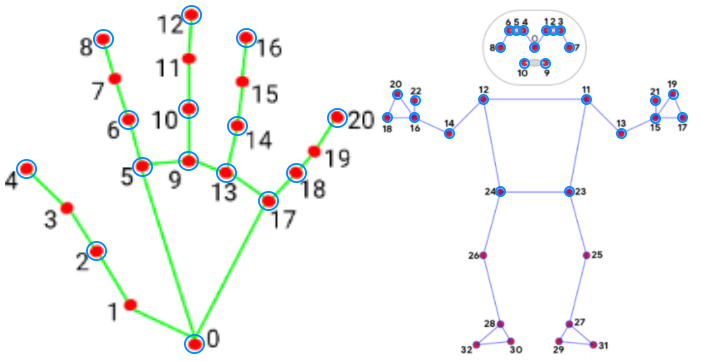
\includegraphics[width=0.6\textwidth]{Graphics/points.png}
    \caption{Todos los puntos obtenidos sin obviar el tren inferior}
    \label{fig:points}
\end{figure}
\subsection{Extraer los datos de la nube}
Utilizando una biblioteca especializada se extraen del almacenamiento en la nube de [\cite{leynier-lsc-2021}]. Por tanto este paso no representa un problema y se logran obtener los datos de dicha investigación anterior para su ulterior uso.
\subsection{Limpieza de los datos}
Los cuadros(frames) del conjunto de datos son variados así que son todos llevados a 24 frames para una mayor homogeneidad del corpus,para agilizar el entrenamiento y porque la estructura neuronal a utilizar requiere de una entrada y una salida de un tamaño fijo.

 A todas las palabras se le hace limpieza con expresiones regulares para eliminar la mayoría de imperfecciones posibles en las palabras, el uso de ''nn'' en lugar de la ''ñ'', presencia de números puesto que al agrupar las frases de varios léxicos distintos, estos se renombraban.
 
 \subsection{Utilizando Embedding de palabra} 
 A pesar de la limpieza se escapaban algunas faltas de ortografía o errores de escritura originados a la hora de teclear dicha frase durante su creación. Es por esto que se recurre a utilizar un modelo de incrustación (embedding) de palabra para exprimir lo máximo posible la información semántica de las frases del corpus [Fig \ref{fig:word2vec}], dada la vérsatilidad del embedding de palabra utilizado el cuál es un modelo cargado pre-entrenado de más de 3 billones de vocablos y caracteres en español cortesía de [\cite{aitor_almeida_2018_1410403}].



\subsection{Extrayendo la matriz de cada frase}
Posteriormente de que se carga el modelo en español del embeddings, se le halla la matriz de tamaño 5x400 a cada frase del corpus. Cada frase contiene un máximo de 5 palabras y como en su mayoría son frases de una sola palabra pues se rellenaba con ceros las filas que no correspondían. Los vectores del embedding son de dimensión 400 por lo que se crea un arreglo de numpy de ceros antes de asignarle los vectores devueltos. 
\subsection{Encontrando similitud de palabras}
Pese a ser un embedding tan potente, en cuanto a cantidad de vocablos con que se entrenó, al ser el idioma tan dependiente de la zona geográfica, como es nuestro caso con el Español, pues en el corpus se encontraron palabras que no tenían representación en el modelo de Word2Vec.

Para solventar dicha situación se recurrió una biblioteca especializada en similitud de palabras para encontrar la palabra más parecida dentro del vocabulario del modelo de embedding.
\subsection{Arreglando errores ortográficos}

Aún así por errores ortográficos (y por inexistencia de algunas) hubo palabras que, al no poseer tilde o estar escritas con mucha falta de ortografía, se tuvieron que codificar a mano en un diccionario de palabras mal escritas dado que eran pocas. Este paso de la solución, dista mucho de ser ideal, pero la similitud de palabras que fueron encontradas pues poseían diferencia semántica muy importante, lo cual afectaría muchísimo al modelo propuesto.

\subsection{Limitando a una sola seña por frase}
Luego de tener el conjunto de frases curadas y limpias, quedaba aún el problema de las palabras repetidas que tienen más de una seña, en dependencia de qué léxico del corpus brindado por el CENDSOR se revise.
Para dicho problema se optó por escoger solamente la primera que apareciera puesto que solo complejizaría más la tarea presentada dado que para una misma frase en el corpus podía incurrir en una variación bastante considerable, es decir la señas para una misma palabra de un intérprete a otro variaban mucho para el caso de la palabra paz con 4 tipos de señas distintas(como si de una ''falta de ortografía'' se tratase). 

\subsection{Inicialización del modelo}Tensorflow y Keras fueron utilizados 
Una vez efectuada la asociación se inicializa el modelo secuencial que consta de 3 capas LSTM, luego a continuación de las anteriores se incluye una capa convolucional de una dimensión, una LSTM, otra 1DConv, otra LSTM y una capa de Reshape para obtener los resultados en las dimensiones esperadas.

El enfoque utilizado en este trabajo para realizar la predicción fue el de utilizar una RNN, específicamente una red de LSTM y además con capas convolucionales. Como se explicó en
la sección \ref{subsection:state-of-the-art:slp:LSTM}, estas son muy utilizadas por su capacidad de recoger información del contexto y las deconvolucionales (convolucionales transpuestas) para ampliar las dimensiones y poder llevar del espacio menor a uno mayor.

No se tuvieron en cuenta los enfoques basados en métodos estadísticos debido a que no
se disponía con un corpus suficientemente preparado y organizado, con sus respectivas
probabilidades para atacar el problema con dichos métodos.

Fueron descartados los enfoques basados en métodos semánticos debido a que  no es del dominio de los autores del trabajo, la estructura gramatical y  semántica de la Lengua de Señas Cubana, siendo
necesaria la ayuda de otros colaboradores, lo cual pertenecía a los objetivos del trabajo en cuestión.

\subsection{Graficación y Animación}
Posteriormente a obtener la matriz de 24 frames con los 67 puntos, de 3 dimensiones cada uno, se utiliza un graficador que está incorporado en el lenguaje utilizado, así como la función utilizada para lograr la animación.
Al ser puntos espaciales , la graficación se realizaba en un ángulo que no era el ideal, para lo cual se realizaron transformaciones para lograr una visualización ideal de la animación con una vista casi frontal,puesto que tiene 1 grado de inclinación, lo cual es despreciable al evaluar el resultado visual.

Dicho resultado se guarda en video en formato mp4 para su ulterior comparación con valores reales similares.
